\section{Intelligent Probing Behavior}
\label{sec:ipro_behavior}

To evaluate the IPro prototype (\textit{cf}. Algorithm 3), its impact (\textit{i.e.,} the change over the time of Probing Interval) in CCO, CUC, and MA (of the throughput) was tested in the test environment described in Section~\ref{sec:setup}. Figure~\ref{fig:load_behavior} depicts the evaluation results, disclosing diverse facts.

%\begin{figure}[htb]
\begin{figure}[h!]
\centering
        \begin{minipage}[t]{1.0\textwidth}
            \centering
            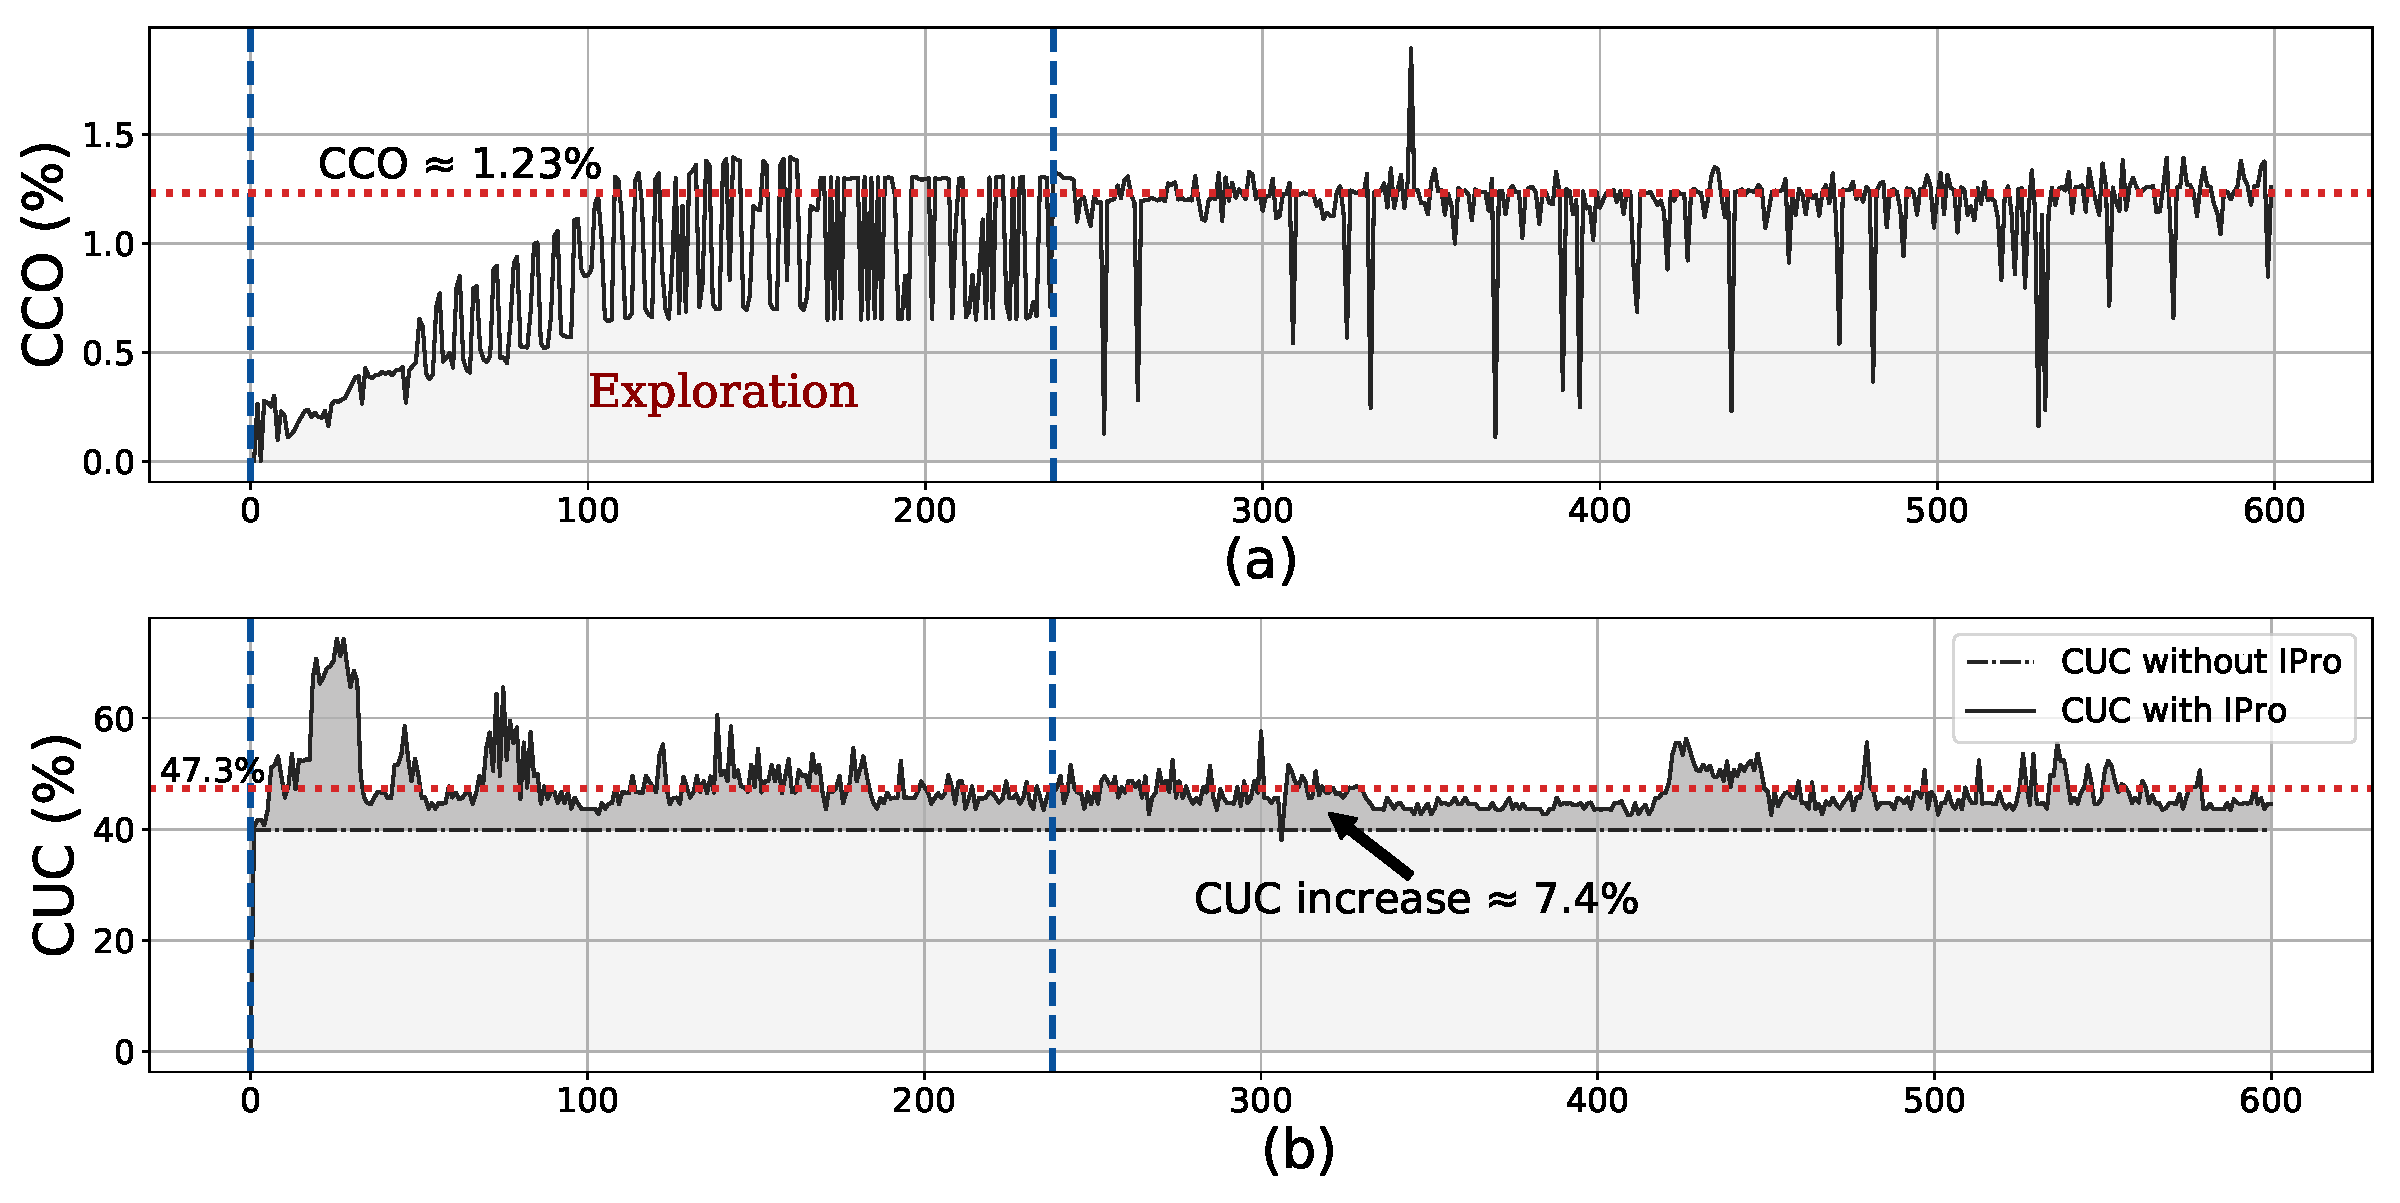
\includegraphics[width=\textwidth]{figures/Figure12a-IPro-behavior-MA-CCO-CUC}
            %\subcaption{Image 1.}\label{fig:1}
        \end{minipage}
        \hfill
        \begin{minipage}[t]{1.0\textwidth}
            \centering
            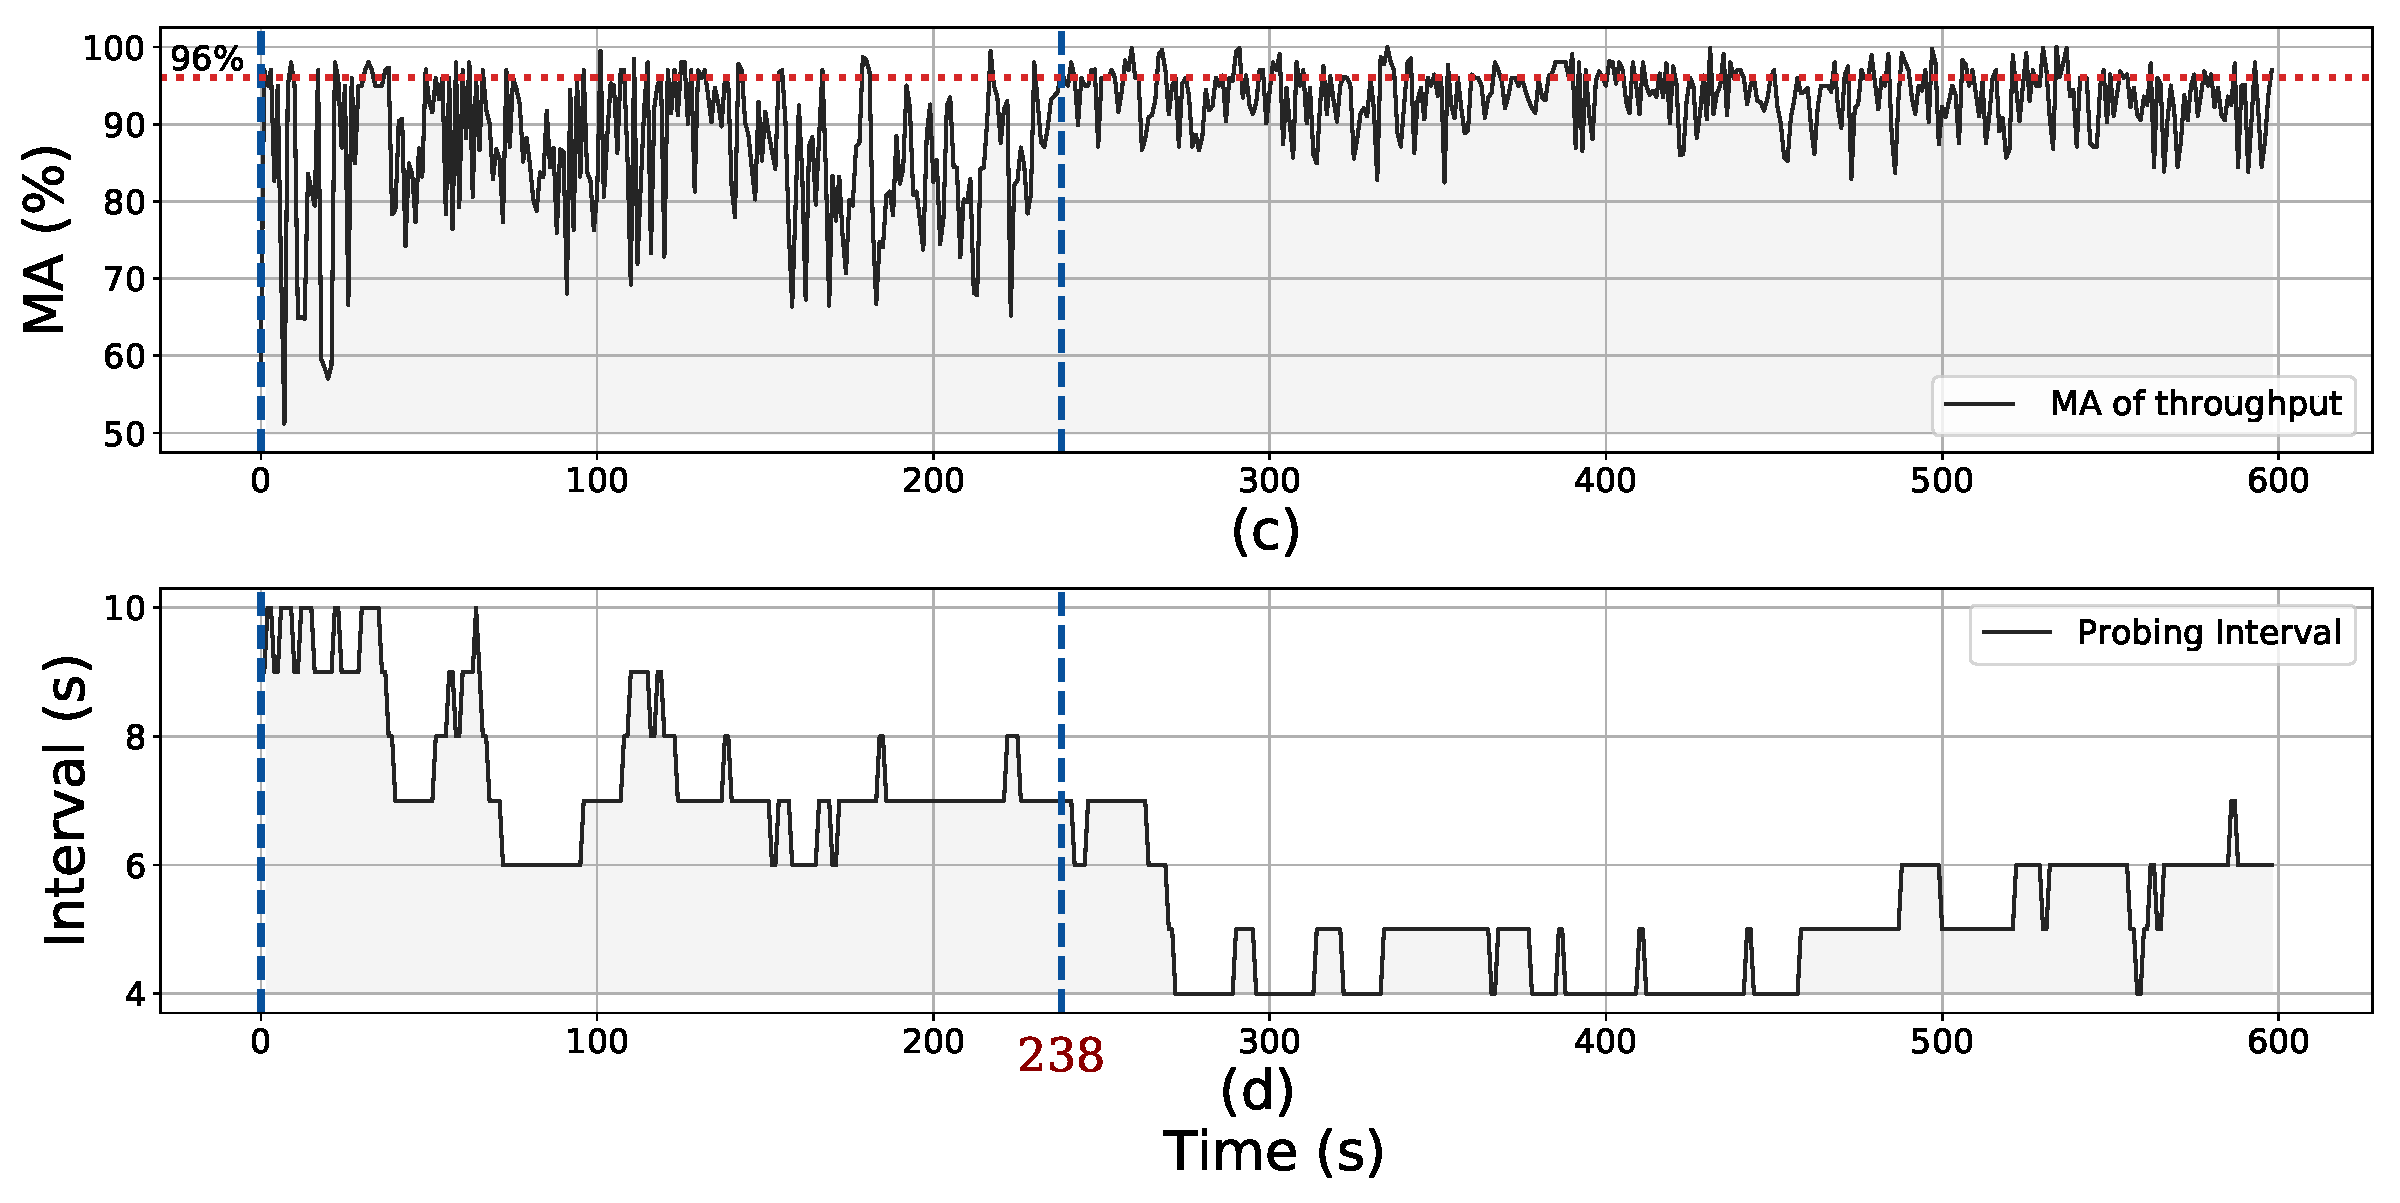
\includegraphics[width=\textwidth]{figures/Figure12b-IPro-behavior-MA-CCO-CUC}
            %\subcaption{Image 2.}\label{fig:2}
        \end{minipage}
        \vspace{-0.5cm}
        \caption{Behavior of the CCO, CUC, MA, and Probing Interval}
        \label{fig:load_behavior}
\end{figure}

\begin{itemize}
    \item During the first 238 seconds (convergence time), CCO, CUC, and MA present a highly fluctuating behaviour Figure~\ref{fig:load_behavior}(a,b,c). This behaviour is because the RL-agent does not have a previous knowledge (\textit{i.e.}, the Q-function starts empty and is filled during this time). Therefore, it is necessary that such an agent starts the exploration process to determine the effect of each action on the network status (\textit{i.e.}, learning process). Figure~\ref{fig:load_behavior}(d) illustrates how the Probing Interval changes during the learning process. As the learning process advances, the RL-agent visits each state of the space of states (\textit{cf.} Equation~\ref{equ:states}) multiple times aiming at finding the most-rewarding probing strategy (\textit{i.e.}, the convergence of the learning process).
    \item After the convergence time, IPro has a CCO near to 1.23\%, a CUC around 7.4\%, and a MA about 96\%. This result demonstrates that, in terms of CCO, CUC, and MA, IPro has good behavior. When the learning process tends to converge, the fluctuations of CCO, CUC, and MA decrease to a smaller radius. This convergence is because a normal distribution function (\textit{cf}. Equation~\ref{equ:reward}) was chosen whereby IPro gradually moves to adjacent states to the target state (\textit{i.e.}, calibrates the action-value function). In particular, IPro provides the best behaviour regarding CCO, CUC, and MA when it probes the network with intervals between 4 and 6 seconds.
    \item It is important to highlight that IPro does not stop its learning because, in real networks, the environment will always be changing and evolving.
\end{itemize}

To determine the performance of IPro itself, the consumption of CPU and memory of its RL-agent was evaluated. Figure~\ref{fig:rl-agent_behavior} depicts the evaluation results, disclosing that this RL-agent does not consume intensively the KP resources, approximately 1\% -2\% of CPU and 30MBytes. These results demonstrate that, in terms of CPU and memory, IPro RL-agent is efficient.

\begin{figure}[h!]
    \centering
    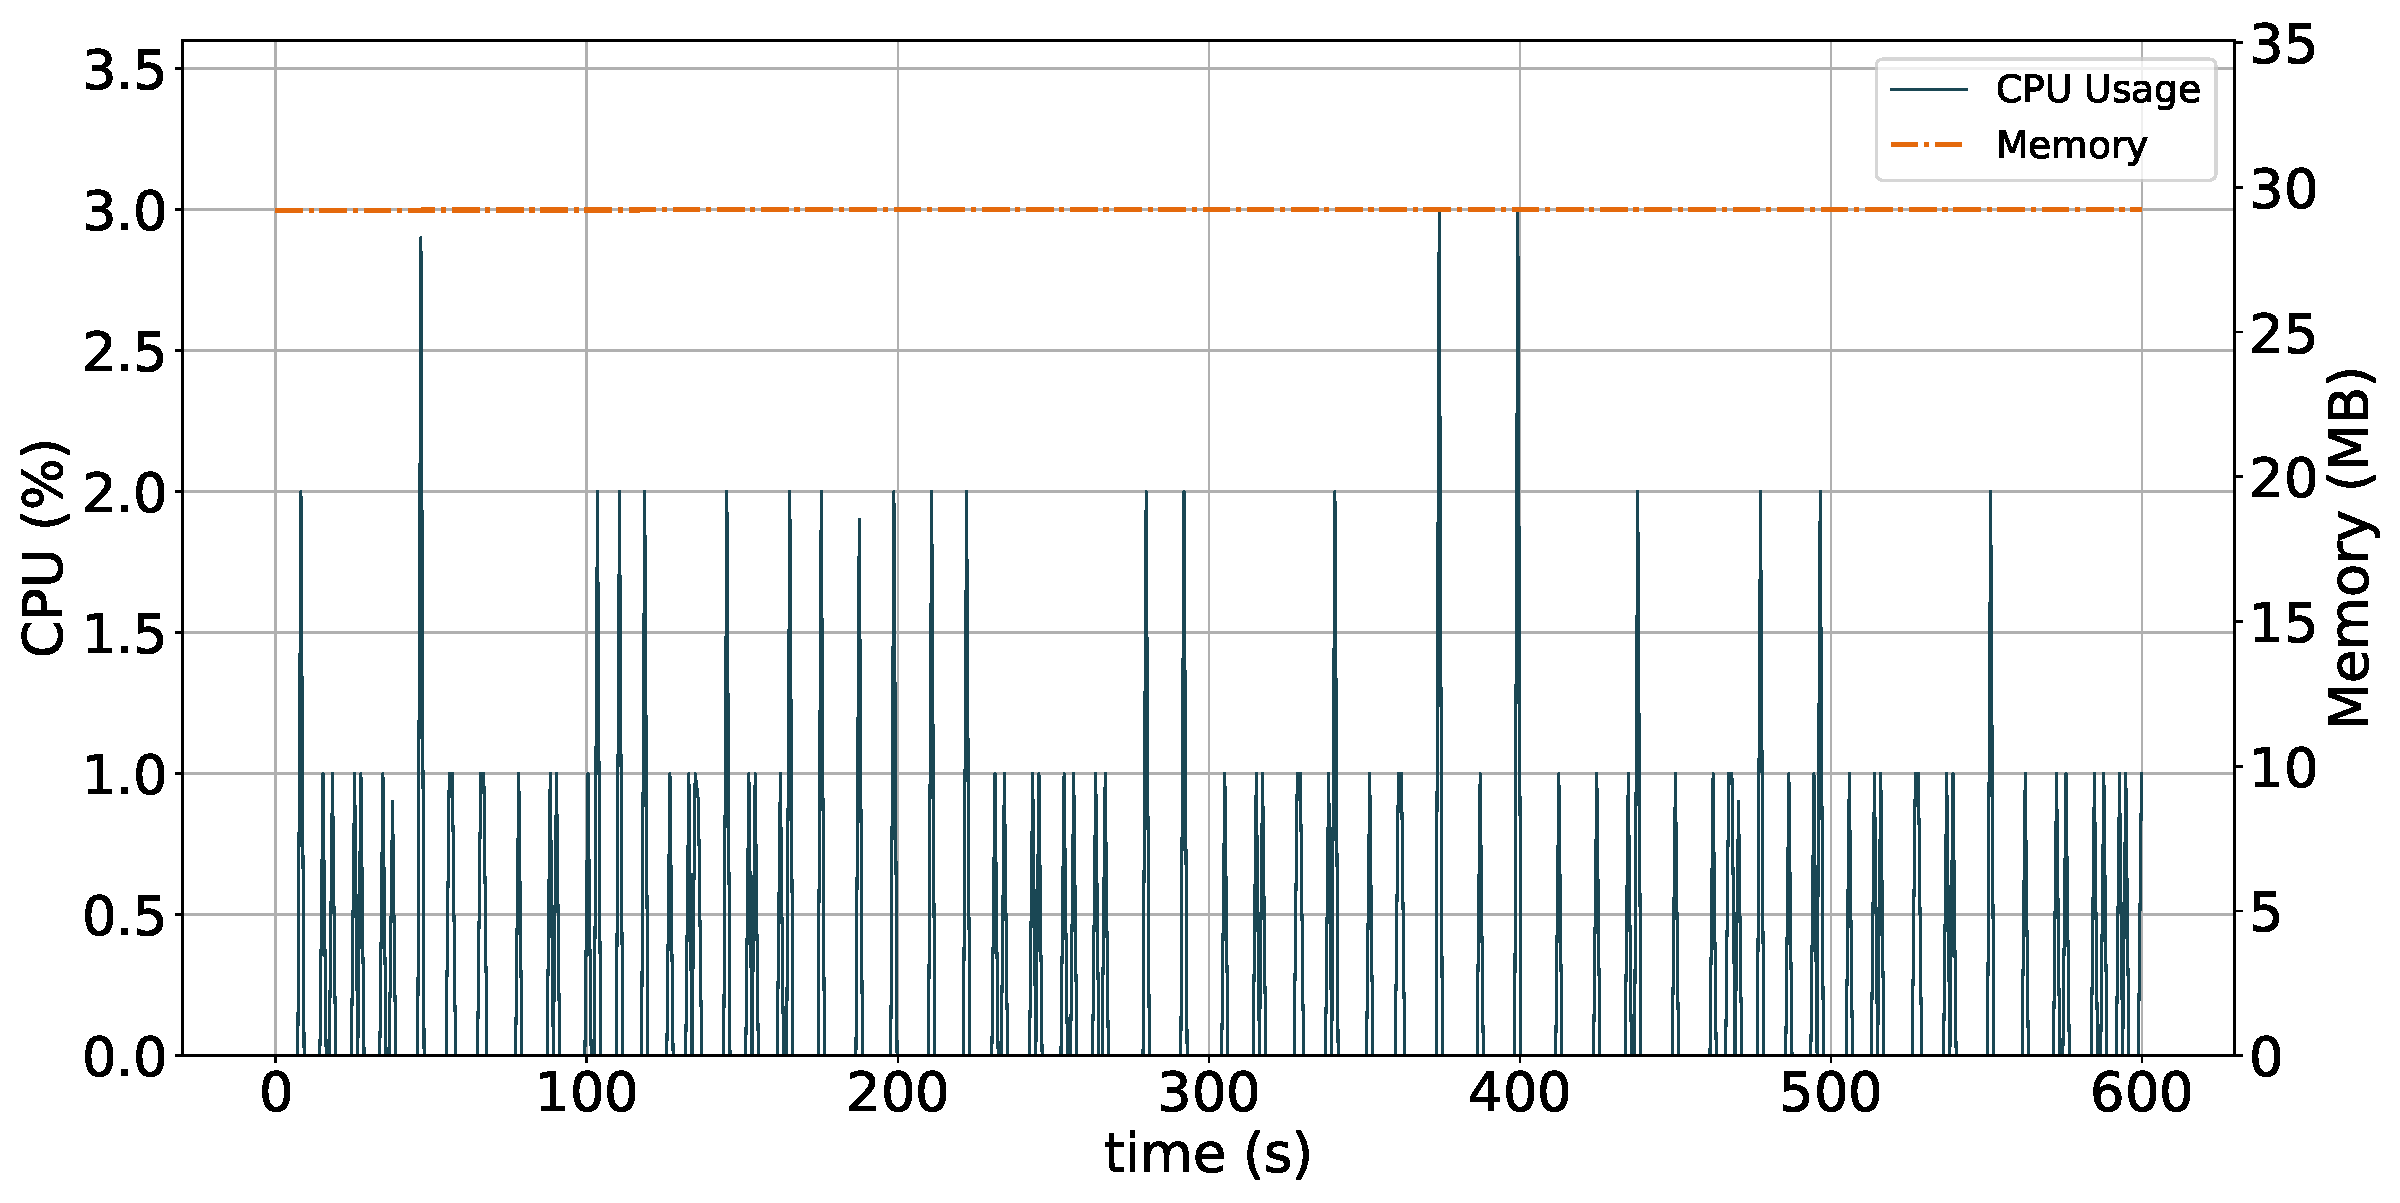
\includegraphics[width=1.0\textwidth]{figures/Figure13-cpu-usage-rl-agent}
    \caption{Behavior of the CPU usage and memory of RL-agent}
    \label{fig:rl-agent_behavior}
\end{figure}